\documentclass{article}

% if you need to pass options to natbib, use, e.g.:
% \PassOptionsToPackage{numbers, compress}{natbib}
% before loading nips_2016
%
% to avoid loading the natbib package, add option nonatbib:
% \usepackage[nonatbib]{nips_2016}

% to compile a development version, don't pass any options.
% \usepackage{nips_2016}

% to compile a camera-ready version, add the [final] option, e.g.:
\usepackage[final]{nips_2016}

\usepackage[utf8]{inputenc} % allow utf-8 input
\usepackage[T1]{fontenc}    % use 8-bit T1 fonts
\usepackage{hyperref}       % hyperlinks
\usepackage{url}            % simple URL typesetting
\usepackage{booktabs}       % professional-quality tables
\usepackage{amsfonts}       % blackboard math symbols
\usepackage{nicefrac}       % compact symbols for 1/2, etc.
\usepackage{microtype}      % microtypography


\usepackage{color,graphicx}
\usepackage{lmodern}
\usepackage{hyperref}
\usepackage{amsmath}
\usepackage{amssymb}
\usepackage[T1]{fontenc}
\usepackage{fancyhdr}
\usepackage{color,graphicx}
\pagestyle{fancy}


\title{Assignment 4}

% The \author macro works with any number of authors. There are two
% commands used to separate the names and addresses of multiple
% authors: \And and \AND.
%
% Using \And between authors leaves it to LaTeX to determine where to
% break the lines. Using \AND forces a line break at that point. So,
% if LaTeX puts 3 of 4 authors names on the first line, and the last
% on the second line, try using \AND instead of \And before the third
% author name.

\author{
  Michele Cer\'u
  %\thanks{Use footnote for providing further
    %information about author (webpage, alternative
    %address)---\emph{not} for acknowledging funding agencies.} 
    \\
 % Department of Computer Science\\
  %Cranberry-Lemon University\\
  %Pittsburgh, PA 15213 \\
  \texttt{mc3784@nyu.edu} \\
}

\begin{document}
% \nipsfinalcopy is no longer used

\maketitle

%\begin{abstract}
 % The abstract paragraph should be indented \nicefrac{1}{2}~inch
  %(3~picas) on both the left- and right-hand margins. Use 10~point
  %type, with a vertical spacing (leading) of 11~points.  The word
  %\textbf{Abstract} must be centered, bold, and in point size 12. Two
  %line spaces precede the abstract. The abstract must be limited to
  %one paragraph.
%\end{abstract}

\section{nngraph}


\begin{figure}[ht!]
  \centering
  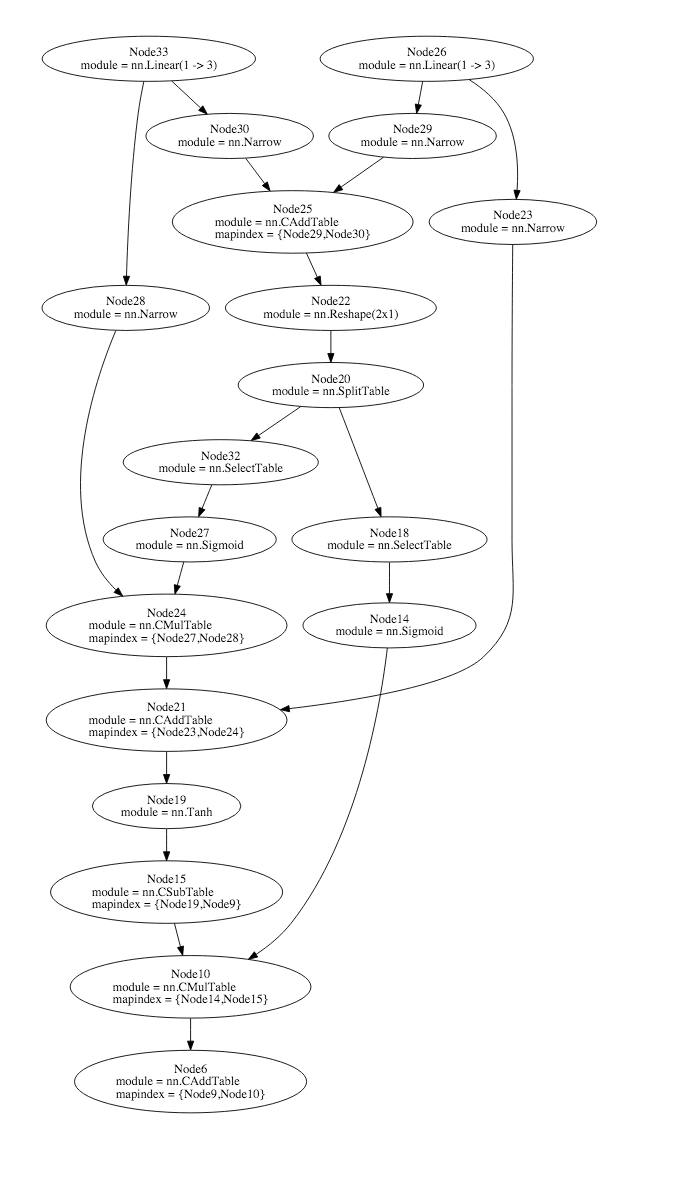
\includegraphics[width=0.50\textwidth]{GRU}
  \caption{ GRU cell graph\label{fig:gru_graph}}
\end{figure}


\section{Language modelling}

\subsection{generating sequences}


\subsection{Suggested improvements to your model}


\begin{center}
\begin{tabular}{ |c|c|c|c|c|c|c|} 
\hline
seq length & layers & rnn size & dropout  & vocab size & best Perplexity\\
\hline
 20 & 2 & 200 & 0 &  10000 & 119.756\\ 
 30 & 2 & 200 & 0 &  10000 & 114.548\\ 
 15 & 2 & 200 & 0 &  10000 & 195.712\\ 
  30 & 4 & 200 & 0 & 10000 & 120.359\\
  40 & 3 & 200 & 0 & 15000 & 137.629\\
  \hline
 40 & 5 & 200 & 0.2 & 10000 & 135.020\\
 40 & 4 & 400 & 0.2 & 10000 & 107.970\\
 30 & 2 & 400 & 0.2 & 10000 & 93.449\\
 30 & 4 & 400 & 0.3 & 10000 & 102.013\\
  30 & 4 & 400 & 0.5 & 10000 & 113.420\\
  
  30 & 2 & 400 & 0.5 &  10000 & 96.340\\
  30 & 2 & 600 & 0.4 &  10000 & 87.368\\  
  30 & 2 & 500 & 0.3 &  10000 & 89.794\\  
   
\hline
\end{tabular}
\end{center}

\begin{center}
\begin{tabular}{ |c|c|c|c|c|c|c|} 
\hline
seq length & layers & rnn size & dropout & vocab size & best Perplexity\\
\hline
 20 & 2 & 200 & 0 &  10000 & 182.217\\ 
 15 & 2 & 200 & 0 &  10000 & 195.712\\ 
 30 & 2 & 600 & 0.4 &  10000 & 97.056\\
 
 30 & 2 & 700 & 0.5 & 10000 & 101.021\\  

\hline
\end{tabular}
\end{center}



\begin{figure}[ht!]
  \centering
  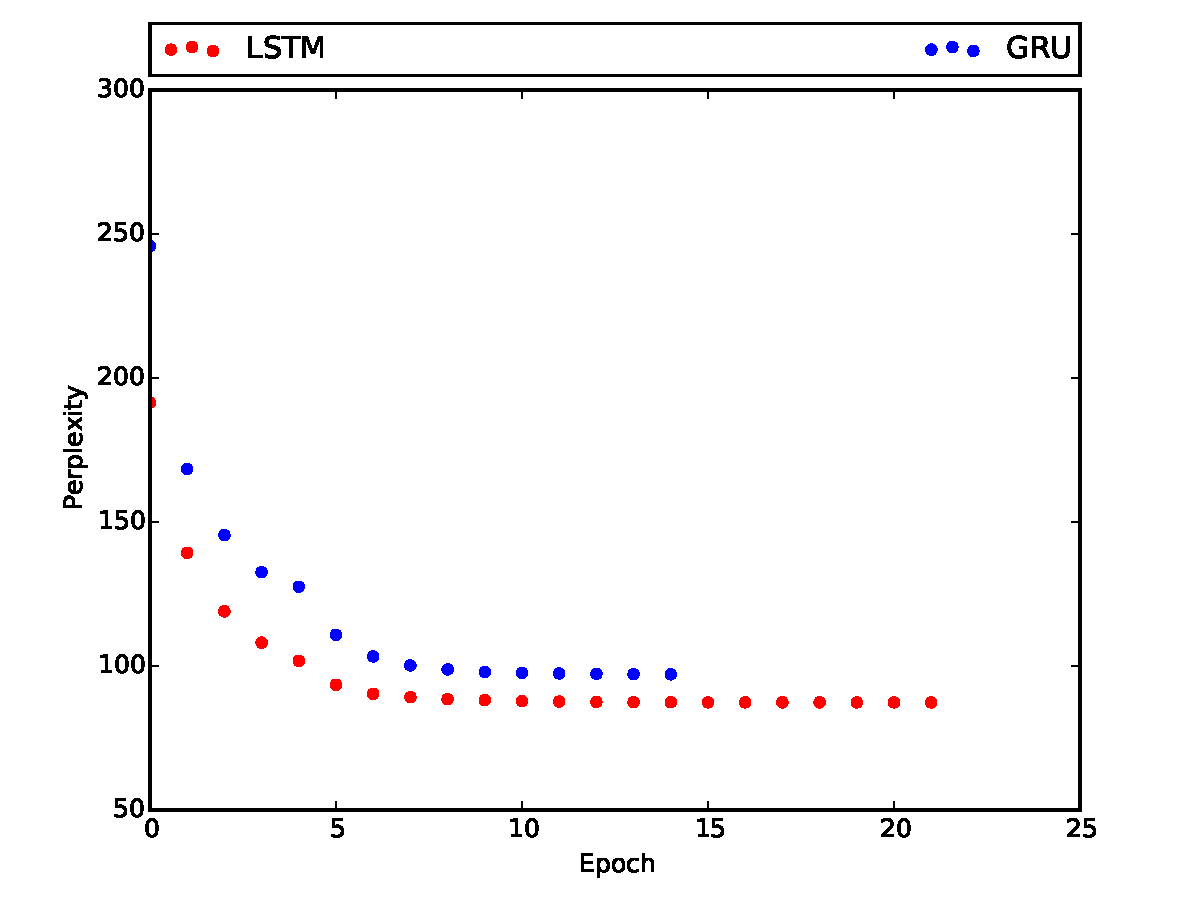
\includegraphics[width=1\textwidth]{LSTMvsGRU.pdf}
  \caption{Second best performance figures. We added a layer that rotates the images by random angles drawn from a normal distribution with zero mean and 0.2 standard deviation. \label{fig:best_performance}}
\end{figure}




\medskip

\small

%[1] Alexander, J.A.\ \& Mozer, M.C.\ (1995) Template-based algorithms
%for connectionist rule extraction. In G.\ Tesauro, D.S.\ Touretzky and
%T.K.\ Leen (eds.), {\it Advances in Neural Information Processing
%  Systems 7}, pp.\ 609--616. Cambridge, MA: MIT Press.



\begin{thebibliography}{9}
\bibitem{bestModel} \url{http://cs.nyu.edu/~mc3784/model.net87.367553621956}
\end{thebibliography} 



\end{document}


